% \documentclass[usenames,dvipsnames]{beamer}
\documentclass[usenames,dvipsnames,handout]{beamer}

\usetheme{AnnArbor}
% \usecolortheme{default}
% \usecolortheme{crane}
\usecolortheme{beaver}
\usecolortheme{dolphin}
% \usecolortheme{orchid}
% \usecolortheme{rose}


\usepackage{fourier}
\usepackage{faktor}
\usepackage{amssymb}
\usepackage{amsmath}
\usepackage{amsthm}
%\usepackage{stmaryrd}
\usepackage{hyperref}
\usepackage[all]{xy}
\usepackage{tikz}
    \usetikzlibrary{mindmap,shadows,shapes.geometric,shapes.misc,positioning}
\usepackage{tikz-cd}
\tikzset{
    invisible/.style={opacity=0},
    visible on/.style={alt={#1{}{invisible}}},
    alt/.code args={<#1>#2#3}{%
      \alt<#1>{\pgfkeysalso{#2}}{\pgfkeysalso{#3}}%
  }
}
%\usetikzlibrary{matrix}
%\usetikzlibrary{calc,intersections}
%\newcommand{\downmapsto}{\rotatebox[origin=c]{-90}{$\large\mapsto$}\mkern2mu} %MnSymbol doesn't work well with beamer
\usepackage{multirow}

\def\Q{\mathbb{Q}}
\def\Z{\mathbb{Z}}
\def\C{\mathbb{C}}
\def\R{\mathbb{R}}
\def\F{\mathbb{F}}

\DeclareMathOperator{\AV}{AV}
\DeclareMathOperator{\Mat}{Mat}
\DeclareMathOperator{\Pol}{Pol}
\DeclareMathOperator{\Char}{char}
\DeclareMathOperator{\rk}{Rank}
\DeclareMathOperator{\Frob}{Frob}
\DeclareMathOperator{\ICM}{ICM}
\DeclareMathOperator{\Pic}{Pic}
\DeclareMathOperator{\Aut}{Aut}
\DeclareMathOperator{\Hom}{Hom}
\DeclareMathOperator{\End}{End}
\DeclareMathOperator{\Gal}{Gal}
\DeclareMathOperator{\mSpec}{mSpec}
\DeclareMathOperator{\GL}{GL}
\DeclareMathOperator{\Tr}{Tr}
\DeclareMathOperator{\Jac}{Jac}
%\renewcommand{\char}{char} %CRASHES WITH beamer
\DeclareMathOperator{\type}{type}


\newcommand{\cG}{\mathcal{G}}
%\newcommand{\cB}{{\mathcal B}}
%\newcommand{\cC}{{\mathcal C}}
\newcommand{\cO}{{\mathcal O}}
\newcommand{\cH}{{\mathcal H}}
%\newcommand{\cM}{{\mathcal M}}
\newcommand{\cT}{{\mathcal T}}
%\newcommand{\cW}{{\mathcal W}}


\newcommand{\vphi}{\varphi}

\newcommand{\p}{{\mathfrak p}}
\newcommand{\frf}{{\mathfrak f}}

\newcommand{\set}[1]{\left\lbrace#1\right\rbrace }
\newcommand{\Span}[1]{\left<#1\right>}

%\newcommand{\AVord}[1]{\AV^{\text{ord}}({#1})}
%\newcommand{\Modord}[1]{\cM^{\text{ord}}({#1})}

%\newcommand{\AVcs}[1]{\AV^{\text{cs}}({#1})}
%\newcommand{\Modcs}[1]{\cM^{\text{cs}}({#1})}

\newcommand{\Acan}{\mathcal{A}_{\mathrm{can}}}
\newcommand{\AcanC}{A_{\mathrm{can}}}
\newcommand{\Palpha}[2]{\mathcal{P}^{\alpha}_{{#1}}({#2})}
\newcommand{\Pone}[2]{\mathcal{P}^{1}_{{#1}}({#2})}

\newcommand{\red}[1]{\textcolor{red}{#1}}
\newcommand{\blue}[1]{\textcolor{blue}{#1}}
\newcommand{\green}[1]{\textcolor{ForestGreen}{#1}}

\newtheorem{df}{Definition}[section]
\newtheorem{remark}[df]{Remark}
\newtheorem{prop}[df]{Proposition}
\newtheorem{cor}[df]{Corollary}

\usepackage{multirow}

%AUTHOR DETAILS
%%%%%%%%%%%%%%%%%%%%%%%%%%%%%%%%%%%%%%%%%%%%%%%%
\title[]{Cohen-Macaulay type of endomorphism rings of\\ abelian varieties over finite fields}
% \subtitle{\onslide<2->{...or...\\when an abelian variety met Bruns-Herzog's book.}}
\author[Stefano Marseglia]{Stefano Marseglia}
\institute[]{University of French Polynesia}
\date[23 May 2024]{Essen Oberseminar - 23 May 2024.}

\begin{document}

\begin{frame}
\titlepage
\end{frame}

\begin{frame}{What do I do for a living?}
    \begin{center}
    \begin{tikzpicture}[
         % squarenodered/.style={rectangle, draw=red!60, fill=red!5, very thick, minimum size=5mm},
         % squarenodeblue/.style={rectangle, draw=blue!60, fill=blue!5, very thick, minimum size=5mm},
         squarenodepurple/.style={rectangle, draw=Black!60, fill=Black!5, very thick, minimum size=5mm},
         % CAlg/.style={rectangle},
         ]
         \onslide<1->{
              \begin{scope}[blend group=darken]
                   \filldraw[color=red!60, fill=red!30] (-2,0) ellipse (3cm and 2cm);
                   \filldraw[color=blue!60, fill=blue!30] (2,0) ellipse (3cm and 2cm);
                   \onslide<4->{\filldraw[color=Orange!60, fill=Yellow!30] (0,-2) ellipse (3cm and 2cm);}
              \end{scope}
              \node (AGset) at (-3,0)
                   {\parbox[c]{4em}{\Large Algebraic\\ Geometry}};
              \node (NTset) at (3,0)
                   {\parbox[c]{4em}{\Large Number\\ Theory}};
         }
         \onslide<4->{
              \node (CAlg) at (-0.5,-2.8)
                   {\parbox[c]{4em}{\centering \Large Commutative \\ Algebra}};   
         }
         \onslide<2->{
                \node[squarenodepurple] (AV) at (-0.5,2.8)    
                     {\parbox[c]{7.5em}{\centering Abelian Varieties: \\ add two points}};
                \draw [-,Black, very thick] (AV.south) .. controls (-0.5,1) ..  (0,0);
         }
         \onslide<3-4>{
                 \node[right=1cm of AV, anchor=west, yshift=-0.5cm] (Abel)
                            {\parbox{3.5cm}{\centering Niels Abel \footnotesize(1802-1829)\\
                                             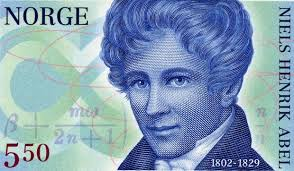
\includegraphics[width=3.5cm]{fig_abel.jpeg}
                            }};
                 \draw [dotted,black,very thick] (Abel) to [out=180,in=0] (AV);
         }
         \onslide<5->{
              \filldraw[color=Black!60, fill=Black!30] (0,0) circle (2cm);
              \node (Comp) at (-0.5,0)
                   {\parbox[c]{4em}{\centering \Large Computations \\ Algorithms}};
              }
         \end{tikzpicture}      
    \end{center}
\end{frame}

\begin{frame}{ Abelian varieties: what are they ? }
\vspace{-0.5cm}
\onslide<1->{Abelian varieties are connected projective group varieties.}
\begin{center}
   \begin{columns}
       \begin{column}{0.4\textwidth}
           \onslide<2->{Abelian varieties of dim.~$1$\\
                           are called {\bf elliptic curves}.\\
                           Eg: over $\R$, $\red{y^2 = x^3 -x +1}$
                           \vspace{1em}}
              % \vpsace{1em}
           \onslide<3->{We can add points:\\
                           $P,Q$ {\Large \blue{$\leadsto$}} $P\oplus Q$
                           \vspace{1em}\\
                           }
              \onslide<4->{Equations are impractical in $\dim \geq 2$.\\
                           We need a better way to represent them...}             
       \end{column}
       \begin{column}{0.5\textwidth}
           \tikz{
               \onslide<2->{
               \draw [help lines] (-2,-2.24) grid (1.8,2.24);
               \draw [->] (-2-0.2,0) -- (1.8+0.2,0) node[right] {$x$}; 
               \draw [->] (0,-2.24-0.2) -- (0,2.24+0.2) node[left] {$y$}; 
               \draw [red, thick, domain=-1.32471795724474602596090885448:1.8, samples=100]
                plot (\x, {sqrt(\x*\x*\x -\x +1)});
               \draw [red, thick, domain=-1.32471795724474602596090885448:1.8, samples=100]
                plot (\x, -{sqrt(\x*\x*\x -\x +1)});
               }
               \onslide<2->{
               \draw [blue, thick, domain=-2:1.8, samples=100] plot (\x, {0.7*\x +0.5 });
               \draw [blue, thick, dashed] (1.3407,2.24) -- (1.3407,-2.24);
               \draw (-1.2858-0.2,-0.7*1.2858+0.5+0.1) node {$P$};
               \draw (0.43506,0.7*0.43506+0.5 +0.3) node {$Q$};
               \draw (1.3407+0.5,-0.7*1.3407-0.5) node {$P\oplus Q$};
               }
           }
       \end{column}
   \end{columns}
\end{center}
\end{frame}

\begin{frame}{ Abelian varieties over $\C$ vs $\F_q$ }    
    \begin{itemize}
     \item Let $A/\C$ be an abelian variety of dimension $g$. 
\pause
    \item Then $A(\C)$ is a {\bf torus}: $T:=\C^g/\Lambda$, where $\Lambda\simeq_\Z\Z^{2g}$.
\pause 
    \item $T$ admits a non-degenerate Riemann form $\longleftrightarrow$ polarization.
\pause
    \item In fact, $ A \mapsto A(\C)$ induces an \blue{equivalence} of categories:
    \vspace{-.2cm}
	  \[
      \set{ \text{abelian varieties $/\C$} } \longleftrightarrow 
      \set{\parbox[c]{12.5em}{\center $\C^g/\Lambda$ with $\Lambda\simeq \Z^{2g}$ admitting\\ a Riemann form}}.
     \]
\pause
    \vspace{-.5cm}
    \item In \red{char.~$p>0$} such an equivalence \red{cannot exist} : there are (supersingular) elliptic curves with quaternionic endomorphism algebras.
\pause 
    \item Nevertheless, as we will see later, over a finite field $\F_q$, we obtain analogous results if we restrict ourselves to certain {\bf subcategories} of AVs.
\pause
    \item WARNING: all morphisms, endomorphisms, isogenies, etc.~are defined over $\F_q$.
	\end{itemize}
\end{frame}

\begin{frame}{ Isogeny classification over $\F_q$}
	\begin{itemize}
    \item An {\bf isogeny} $A\to B$ is a surjective morphism with finite kernel.
\pause     
    \item $A/\F_{q}$ comes with a {\bf Frobenius} endomorphism, 
\pause
    that induces an action
		\[ \Frob_A : T_\ell A \rightarrow T_\ell A \text{ for any }\ell\neq p, \]
		where $T_\ell(A) = \varprojlim A[\ell^n] \simeq \Z_\ell^{2g}$.
\pause
    \item $\blue{h_A(x)}:=\Char(\Frob_A)$ is a \blue{$q$-Weil} polynomial.
\pause
    \item {\bf Honda-Tate} theory:\\
        - $h_A(x)$ is *the* {\bf isogeny invariant} 
        \[ A\sim_{\F_q} B \text{ iff } h_A(x) = h_B(x), \]
\pause
        - the association
		\[ \text{isogeny class of }A \longmapsto h_A(x) \]
		allows us to \blue{enumerate} all AVs up to isogeny.
	\end{itemize}
\end{frame}

\begin{frame}{ Endomorphism rings }
	\begin{itemize}
    \item $\End_{\F_q}(A)$ is a free $\Z$-module of finite rank ... 
\pause 
    \item ... $\End_{\F_q}(A) \subset \End_{\F_q}(A)\otimes_\Z\Q$.
\pause 
    \item Denote by $\pi_A\in \End_{\F_q}(A)$ the Frobenius endomorphism of $A$.
\pause 
    \item Tate: $h_A(x)$ is squarefree $\iff$ $\End(A)$ is commutative.\\
    (We will assume this for the rest of the talk.)
\pause 
    \item Set $K=\Q[x]/(h_A) = \Q[\pi]$. It is an {\bf \'etale $\Q$-algebra}\\
    (i.e.~a finite product of number fields).
\pause 
    \item The association $\pi_A \mapsto \pi$ allows us to identify $\End(A)$ with a special kind of subring of $K$:
\pause 
    \item $\Z[\pi,q/\pi] \subseteq \End_{\F_q}(A) \subseteq \cO_K$ are orders in $K$\\
    (an {\bf order} $R$ in $K$ is a subring $R\subset K$ such that $R\simeq_\Z \Z^{\dim_\Q K}$).
\pause 
    \item 
    \red{Plan}: study $A$ by studying some comm.~algebra properties of $\End(A)$.
	\end{itemize}
\end{frame}

% \begin{frame}{ Abelian varieties : Introduction } 
%     \begin{itemize}
%     \item Let $A$ be an {\bf abelian variety} over $\F_q$, $q=p^a$, of dimension $g$.
%     \item \pause $\End_{\F_q}(A)$ is a free $\Z$-module of finite rank ... 
%     \item \pause ... $\End_{\F_q}(A) \subset \End_{\F_q}(A)\otimes_\Z\Q$.
%     \item \pause Denote by $\pi_A\in \End_{\F_q}(A)$ the Frobenius endomorphism of $A$... 
%     \item \pause ... and by $h_A(x)$ the {\bf characteristic polynomial} of $\pi_A$ acting on 
%         \[ \pi_A	\curvearrowright T_\ell A = \varprojlim A[l^n] \simeq_{\Z_\ell} \Z_\ell^{2g}, \quad \text{for a prime }\ell \neq p. \]
%     \item \pause Ex. $E/\F_5 : Y^2 = X^3 + X \rightsquigarrow h_{E}(x) = x^2 - 2x + 5$.
%     \item \pause Ex. $C/\F_3: Y^2=X^6+X+1 \rightsquigarrow h_{\Jac(C)}(x) = 
%     x^4 + 3 x^3 + 6 x^2 + 9 x + 9$. 
% 	\end{itemize}
% \end{frame}

% \begin{frame}{ Abelian varieties : endomorphism algebra } 
%     \begin{itemize}
%     \item Some facts (Tate + Weil conjectures):
%         \begin{itemize}
%             \item \pause $h_A$ does not depend on the choice of $\ell$.
%             \item \pause $h_A \in \Z[x]$ of degree $2g$.
%             \item \pause $A/\F_q$ and $B/\F_q$ are $\F_q$-isogenous $\iff h_A=h_B$.
%             \item \pause $h_A$ is squarefree (i.e.~no repeated $\C$-roots) $\iff \End_{\F_q}(A)$ is commutative. 
%         \end{itemize}
%     \item From now on:
%         \begin{itemize}
%             \item \pause We assume that $h_A$ is {\bf squarefree}.
%             \item \pause We identify $\End_{\F_q}(A)\otimes_\Z\Q = \Q[x]/h_A=\Q[\pi]$ by $\pi_A \mapsto \pi$.
%         \end{itemize}
%     \item Note:
%         \begin{itemize}
%             \item \pause $K=\Q[\pi]$ is a {\bf \'etale $\Q$-algebra}\\
%             (i.e.~a finite product of number fields).
%             \item \pause $\Z[\pi,q/\pi] \subseteq \End_{\F_q}(A) \subseteq \cO_K$ are orders in $K$\\
%             (an {\bf order} $R$ is a subring $R\subset K$ such that $R\simeq_\Z \Z^{\dim_\Q K}$).
%         \end{itemize}    
% 	\end{itemize}
% \end{frame}

\begin{frame}{ Orders and fractional ideals in \'etale $\Q$-algebras } 
    \begin{itemize}
    \item \pause Let $R$ be an order in a \'etale $\Q$-algebra $K$.
    \item \pause A {\bf fractional $R$-ideal} is a sub-$R$-module $I\subset K$ such that $I\simeq_\Z\Z^{\dim_\Q K}$.
    \item \pause Given fr.~$R$-ideals $I,J$ then 
    $$(I:J)=\set{a \in K : aJ\subseteq I}
    \quad \text{and}\quad I^t=\set{a \in K : \Tr_{K/\Q}(a I)\subseteq \Z}$$
    are also fr.~$R$-ideals.
    \item \pause We have $(I:I)^t = I\cdot I^t$.
    \item \pause A fr.~$R$-ideal $I$ is invertible if $I(R:I)=R$ ...
    \item \pause ... or, equivalently, $I_\p \simeq R_\p$ as $R_\p$-modules for every $\p$ maximal $R$-ideal.\\
        ($R_\p$ is the completion of $R$ at $\p$)
    \item \pause If $I$ is invertible, then $(I:I)=R$.
	\end{itemize}
\end{frame}

\begin{frame}{ Cohen-Macaulay type and Gorenstein orders } 
    \begin{itemize}
    \item Def: The {\bf (Cohen-Macaulay) type} of $R$ at a maximal ideal $\p$ is
        \[ \type_\p (R) := \dim_{R/\p} \frac{R^t}{\p R^t}. \]
    \item \pause Def: $R$ is {\bf Gorenstein} at $\p$ if $\type_\p(R)=1$.
    \item \pause Remark: these definitions coincides with the 'usual' ones.
    \item \pause Ex: monogenic $\Z[\alpha]$ and maximal $\cO_K$ orders are Gorenstein.\\
    (also $\Z[\pi,q/\pi]$ for AVs).
    \item \pause Ex: pick a prime $\ell\in\Z$. Then $\type_{\ell\cO_K}(\Z+\ell\cO_K) = \dim_\Q K-1$.
	\end{itemize}
\end{frame}

\begin{frame}{ Classification for orders of type $\leq 2$ } 
    \begin{theorem}
        Let $\p$ be a maximal ideal of $R$, and $I$ a fr.~$R$-ideal with $(I:I)=R$.
        \begin{enumerate}
            \item \pause If $\type_\p(R)=1$ (Gorenstein) then $I_\p\simeq R_\p$ as $R_\p$-modules.
            \item \pause If $\type_\p(R)=2$ then either $I_\p\simeq R_\p$ or $I_\p\simeq R^t_\p$  as $R_\p$-modules.
        \end{enumerate}
    \end{theorem}

    \pause Part 1 is contained (in a much more general form) in the "Ubiquity" paper by H.~Bass.\\
    Part 2 is new, and we give a proof.
    \pause 
\begin{lemma}
    Let $U,V,W$ be vectors spaces (over some field). Assume that $\dim W \ge 2$, and let $m: U\otimes V\to W$ be a surjective map. Then:
    \begin{enumerate}
        \item \pause $\exists u\in U$ such that $\dim(m(u\otimes V)) \ge 2$, or
        \item \pause $\exists v\in V$ such that $\dim(m(U\otimes v)) \ge 2$.
    \end{enumerate}
\end{lemma}

\end{frame}


\begin{frame}{ Proof of Part 2 } 
    \begin{itemize}
    \item \pause Put $U = I/\p I$, $V = I^t/\p I^t$ and $W = R^t/\p R^t$.
    \item \pause By assumption $R^t = I \cdot I^t$, so the map $ m: U \otimes V \to W $ induced by multiplication $I \times I^t \to R^t$
    is surjective.
    \item \pause Moreover, $\dim W = 2$ (because of the assumption on the type).
    \item \pause By the Lemma:
    \begin{enumerate}
        \item $\exists x \in I$ such that $m( (x+\p I) \otimes V  ) = \frac{x I^t + \p R^t }{ \p R^t }$ equals $W$.\\
            By Nakayama's lemma: $I_\p^t\simeq R_\p^t \iff R_\p\simeq I_\p $,...
        \item \pause ...or, $\exists y \in I^t$ such that $U \otimes m( U \otimes (y+\p) I^t ) = W $ implying $I^t_\p \simeq R_\p \iff I_\p \simeq R^t_\p$.
    \end{enumerate}
	\end{itemize}
\end{frame}

\begin{frame}{ Back to AVs: Categorical equivalence(s) }
    Fix a squarefree characteristic poly $h(x)$ of Frobenius $\pi$ over $\F_q$.\\
    Put $K=\Q[x]/h=\Q[\pi]$.\\
    Let $\mathcal{I}_h$ be the corresponding isogeny class.
    \pause 
    \begin{theorem}
        Assume that $q=p$ is prime or that $\mathcal{I}_h$ is ordinary.\\
        \pause Then there is an {\bf equivalence} of categories
        \[
        \begin{array}{cc}
        & \set{ \text{ $\mathcal{I}_h$ with $\F_q$--morphisms } }  \\
        & \updownarrow \\ 
        & \set{ \text{fr.~$\Z[\pi,q/\pi]$-ideals with linear morphisms} }
        \end{array} 
        \]  
        \pause Moreover, if $A\mapsto I$ then $A^\vee \mapsto \overline{I}^t$, where $\overline{\cdot}$ is defined by $\overline{\pi}=q/\pi$ (the CM-involution).
    \end{theorem}
    \pause References: Deligne, Howe, Centeleghe-Stix, Bergstr\"om-Karemaker-M.
\end{frame}

\begin{frame}{ AVs: Isomorphism classes }

\end{frame}

\begin{frame}{ AVs: Group of rational points }

\end{frame}

\begin{frame}{ AVs: self-duality }
    \begin{theorem}[ Springer-M. ]
        $\mathcal{I}_h$ and $K=\Q[\pi]=\Q[x]/h$ as before.\\
        \pause Let $R$ be an order in $K$ and $\p$ a maximal ideal of $R$ (possibly but not necessarily above $p$). 
        \pause Assume:
        \[ R=\overline{R}, \quad \p = \overline{\p},\quad \text{and}\quad \type_\p(R) = 2 .\]
        \pause Then for every $A \in \mathcal{I}_h$ such that $\End(A)=R$ we have that $A\not\simeq A^\vee$. 
        \pause In particular, such an $A$ cannot be principally polarized nor a Jacobian.
    \end{theorem}
    \pause Proof: Say that $A \mapsto I$. Hence $A^\vee \mapsto \overline{I}^t$.\\
    \pause By the Classification: either $I_\p\simeq R_\p$ or $I_\p\simeq R_\p^t$.\\
    \pause In the first case: $\overline{I}_\p^t = \overline{I}_{\overline{\p}}^t \simeq R^t_\p \not\simeq R_\p$.\\
    \pause Similarly, in the second: $\overline{I}_\p^t = \overline{I}_{\overline{\p}}^t \simeq R_\p \not\simeq R_\p^t$.\\
    \pause In both cases: $I\not\simeq \overline{I}^t \iff A\not \simeq A^\vee$.
\end{frame}

\begin{frame}{ Some stats and refs }
    \red{Be more precise in this slide\\}
    Soon on the LMFDB there will be tables of isomorphism classes of AVs$/\F_q$.
    \pause Over $615269$ isogeny classes for $1\leq g \leq 5$ and various $q$, we encountered
    \begin{itemize}
        \item $3.914.908$ commutative endomorphism rings, of which:
        \item \pause $72.6 \%$ satisfy $R=\overline{R}$;
        \item \pause $10.3 \%$ satisfy $R=\overline{R}$ and are non-Gorenstein;
        \item \pause $7.4 \%$ satisfy $R=\overline{R}$, are non-Gorenstein and the Theorem applies.
	\end{itemize}
\end{frame}

\begin{frame}{  }
    \begin{center}
    \green{\huge Thank you!}
    \end{center}
    \pause 
    {\footnotesize References:
    \begin{itemize}
        \item \emph{Cohen-Macaulay type of orders, generators and ideal classes}\\
            \url{https://arxiv.org/abs/2206.03758}
        \item \emph{Abelian varieties over finite fields and their groups of rational points}\\
            with Caleb Springer,\\
            \url{https://arxiv.org/abs/2211.15280}
        \item Magma package for \'etale $\Q$-algebras\\
            \url{https://github.com/stmar89/AlgEt} 
            (also in Magma 2-28.1)
    \end{itemize}
    }
\end{frame}

% \begin{frame}[noframenumbering]{ Secret Slide }
	
% \end{frame}

\end{document}
